\documentclass[11pt]{article}
\usepackage[utf8]{inputenc}
\usepackage[T1]{fontenc}
\usepackage[margin=2.5cm]{geometry}
\usepackage{amsmath,amssymb}
\usepackage{graphicx}
\usepackage{booktabs}
\usepackage{xcolor}
\usepackage[hidelinks]{hyperref}
\usepackage[numbers,sort&compress]{natbib}

\graphicspath{{../results/figures/}}
\newcommand{\todo}[1]{\textcolor{red}{[TODO: #1]}}

\title{Coordinating learned one-dimensional solvers:\\
assembling 2D and 3D elliptic solutions from a single 1D neural network}
\author{Artemii-Denys Vitiuk}
\date{\today}

\begin{document}
\maketitle

\begin{abstract}
We study a coordination (dimension-splitting) method in which a multidimensional
elliptic problem is decomposed into independent one-dimensional subproblems, one family
per coordinate direction, coupled through an unknown coordinator field $q$ that is chosen
so that all subproblem states agree. The method only ever \emph{solves} subproblems; it
never applies the multidimensional operator. This makes it a natural host for learned
(neural) subproblem solvers. We show that (i) the error of the assembled solution is not
amplified relative to the error of the 1D solver (empirical amplification $0.3$--$1.05$);
(ii) a single hybrid 1D network, trained for about four minutes on a laptop CPU only on 1D
lines of 24--96 nodes, solves variable-coefficient diffusion problems on $50^2$--$200^2$
grids with $0.55\%$ mean error and on $24^3$--$96^3$ grids (up to $8.8\cdot10^5$ unknowns) with
$0.36$--$0.49\%$ mean error, without ever seeing 2D or 3D data; (iii) the subproblem surrogate
must be accurate uniformly in frequency, which a standard Fourier neural operator fails and
an analytic-prior-plus-learned-correction design satisfies; (iv) against a 2D Fourier neural operator
trained on 2D solutions, coordination with a residual-refined 1D network has $0.05$--$0.7\%$ mean error on every tested grid and
boundary type versus $3.5$--$9.9\%$, while being 40--60 times slower at inference; (v) a nonlinear ``atmospheric
column'' with second-order chemistry can be replaced by a network that predicts an effective
reaction rate, coupled to a classical horizontal solver, with $0.1$--$3.9\%$ error depending on
the strength of the chemistry; (vi) for three reacting species (NO--NO$_2$--O$_3$), a network that predicts the
ozone profile is an effective warm start for Newton's method: with three Newton steps it reaches machine
precision and makes column solves 1.9--3.2 times faster, although in the steady coupled problem the run time
is dominated by the coupling iterations. We also report, for transparency, that with exact 1D solvers
the coordination method preconditioned by ADI is equivalent to ADI-preconditioned GMRES on
the original problem and is not faster. All code and logs are available.
\end{abstract}

\section{Introduction}

Neural surrogates for partial differential equations are typically trained on solutions of
the full multidimensional problem~\cite{li2021fno}. Generating such data is expensive, and a
model trained on one grid, geometry or boundary-condition family often transfers poorly.
Hybrid approaches therefore couple neural components with classical solvers, for example in
Schwarz domain decomposition with neural subdomain solvers~\cite{lddm2025,femdeeponet2025},
neural subdomain solvers used as preconditioners in multilevel domain decomposition~\cite{fan2025neuralprecond}, or neural operators for individual
fractional steps of operator-splitting schemes~\cite{nos2026,dosnet2022}. In weather and
climate modelling, learned \emph{column} parameterisations are coupled to a classical
dynamical core~\cite{neuralgcm2024,climsim2023}; stable coupling is a known difficulty.

We consider a different decomposition: by \emph{coordinate direction}. A $d$-dimensional
elliptic operator $L = X_1 + \dots + X_d$ is split into one-dimensional operators acting along
grid lines, and the subproblems are coupled by a coordinator field. Each subproblem is a batch
of independent 1D problems, so a single 1D model can serve every direction, every grid size
and every dimension. Our contributions are:
\begin{itemize}
  \item an analysis and measurements showing that coordination does not amplify subproblem
        errors, with exact, synthetically perturbed and learned 1D solvers;
  \item a hybrid 1D solver (analytic high-frequency prior plus a learned low-mode correction,
        exactly linear in the source) that transfers across grid sizes and from 1D to 2D and 3D;
  \item the observation that surrogate accuracy must be uniform in frequency, illustrated by
        the failure of a standard 1D FNO inside the coordination loop;
  \item a nonlinear chemistry-column demonstration in which only the vertical column is
        learned, with a classical horizontal solver;
  \item a three-species (NO--NO$_2$--O$_3$) column in which the network is used as a warm start for
        Newton's method, reaching machine precision with 1.9--3.2 times faster column solves
        (Section~\ref{sec:multi});
  \item residual refinement with a network fine-tuned through the unrolled refinement, which removes the
        loss of accuracy at high coefficient contrast up to $\approx50$;
  \item a comparison with a 2D FNO trained on 2D solutions: 30--180 times lower mean error on all tested grids
        and boundary types, at higher inference cost (Section~\ref{sec:baseline}).
\end{itemize}

\section{The coordination method}
\label{sec:method}

The coordination formulation used here originates from earlier unpublished diploma work on
coordinating one-dimensional subproblems; the present paper builds on it, replacing the 1D
subproblem solvers by neural networks and extending it to 3D and to nonlinear chemistry columns.

Consider $-\nabla\cdot(k\nabla\varphi) = s$ on $\Omega = (0,1)^2$ with Dirichlet data, and
its standard five-point discretisation $L\varphi = (X+Y)\varphi = b$, where $X$ ($Y$) collects
the second differences along $x$ ($y$) grid lines. Introduce the coordinator $q$ and the
subproblem states
\begin{equation}
  X u = b_x - q, \qquad Y v = b_y + q, \qquad b_x + b_y = b. \label{eq:split}
\end{equation}
If $u = v$, then $(X+Y)u = b$, i.e.\ $u = v = \varphi$. The coordinator is therefore defined by
\begin{equation}
  R(q) = u(q) - v(q) = c - Mq = 0,\qquad M = X^{-1} + Y^{-1} = X^{-1}(X+Y)Y^{-1}. \label{eq:coord}
\end{equation}
Each evaluation of $R$ requires one batch of independent line solves along $x$ and one along
$y$; $M$ is never formed. We solve~\eqref{eq:coord} with GMRES~\cite{saad1986gmres}. In $d$
dimensions there are $d-1$ independent coordinators, e.g.\ in 3D
$X u_1 = q_1$, $Y u_2 = q_2$, $Z u_3 = -q_1 - q_2$ (plus boundary data), with residuals
$u_1-u_3$, $u_2-u_3$.

\paragraph{Preconditioning and a negative result.}
With $P = Y A_m X$, where $A_m \approx (X+Y)^{-1}$ is $m$ Peaceman--Rachford (ADI)
steps~\cite{peaceman1955}, one obtains $MP = X^{-1}[(X+Y)A_m]X$, which is \emph{similar} to the
ADI-preconditioned original operator. Hence coordination with this preconditioner needs the
same number of GMRES iterations as ADI-preconditioned GMRES applied directly to $L\varphi=b$,
and is slower because each iteration does more line solves. We verified this numerically
(Table~\ref{tab:adi}). Without preconditioning, $\mathrm{cond}(M)\approx\mathrm{cond}(X+Y)$.
The interest of coordination is therefore not speed with exact solvers, but \emph{modularity}:
it needs only a subproblem solver, which may be a black box.

\begin{table}[t]
\centering
\caption{Exact 1D solvers, Laplace equation, CPU float64: coordination with ADI preconditioning
versus GMRES with the same ADI preconditioner on the original five-point problem.}
\label{tab:adi}
\begin{tabular}{rrrrr}
\toprule
grid & coordination & iterations & direct GMRES+ADI & iterations\\
\midrule
$100^2$ & 0.027 s & 6 & 0.012 s & 6\\
$400^2$ & 0.241 s & -- & 0.155 s & --\\
$800^2$ & 2.19 s & -- & 1.68 s & 9\\
\bottomrule
\end{tabular}
\end{table}

\paragraph{Learned subproblem solvers.}
Replace $X^{-1}$ and $Y^{-1}$ by surrogates $N_X$, $N_Y$. Then $R(q) = N_X(b_x-q) - N_Y(b_y+q)$
may be nonlinear in $q$ and is solved by Newton--Krylov~\cite{knoll2004jfnk}, with Jacobian--vector
products computed by forward-mode automatic differentiation. If the surrogate is exactly linear
in its source term, $R$ is affine and a single GMRES solve suffices.

\section{Error amplification}
\label{sec:amplification}

We first perturb the exact line solver multiplicatively, $\tilde N(r) = X^{-1}r\odot(1+\varepsilon z)$,
with $z$ either white noise or a smooth field, and solve~\eqref{eq:coord} to convergence. The
relative error of the assembled solution equals $0.82\,\varepsilon$ (white) and $0.28\,\varepsilon$ (smooth)
for $\varepsilon\in\{10^{-1},10^{-2},10^{-3}\}$ and grids $50^2$--$400^2$, i.e.\ it is independent of the
grid even though $\mathrm{cond}(M)=O(h^{-2})$. Figure~\ref{fig:amp} collects this and the
learned-solver experiments below: in all cases the solution error is at most the subproblem error.

\begin{figure}[t]
\centering
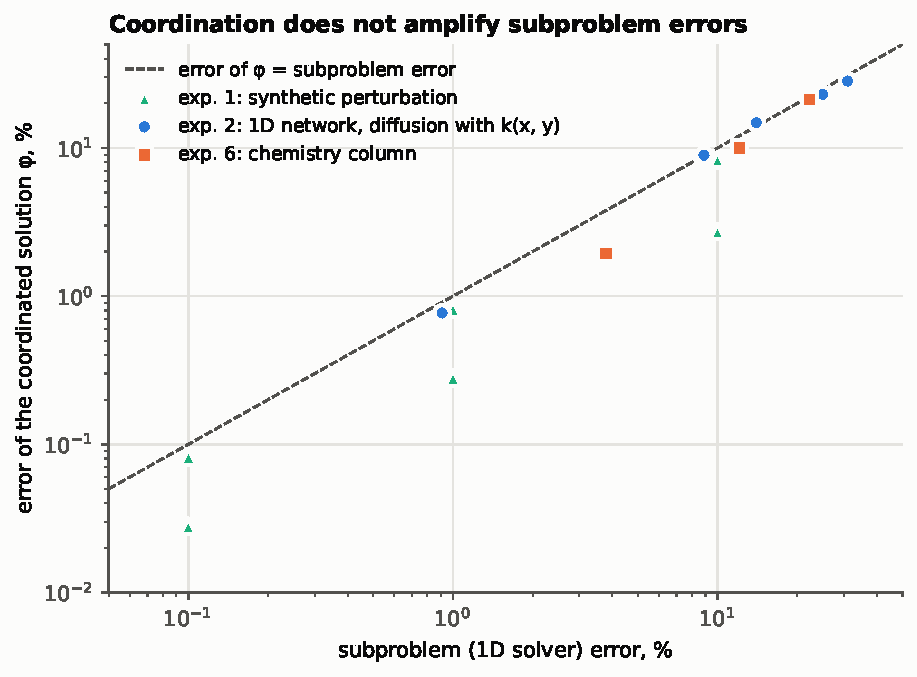
\includegraphics[width=0.62\linewidth]{fig4_error_amplification}
\caption{Error of the assembled solution versus error of the 1D subproblem solver (on the inputs it
actually receives). Dashed: equality.}
\label{fig:amp}
\end{figure}

\section{A grid-independent hybrid 1D solver}
\label{sec:hybrid}

The 1D subproblem is $-(c\,u')' = f$ on $(0,1)$, $u(0)=a$, $u(1)=b$, with $c$ given at half-nodes.
The homogeneous part (boundary data) is computed exactly; a network handles the part with zero
boundary values.

\paragraph{Why a standard neural operator fails.}
A 1D Fourier neural operator in a sine basis reached $0.3$--$0.5\%$ relative $L^2$ error on lines of
any length (32--512 nodes) but produced $7$--$415\%$ error inside the 2D coordination loop. The
cause is spectral (Figure~\ref{fig:freq}): its error for $f=\sin k\pi x$ grows from $0.4\%$ at $k=1$
to $270\%$ at $k=47$. The $L^2$ norm hides this, since the response to high frequencies is small
($\sim k^{-2}$), but the coordination operator and its preconditioner weight all frequencies.
\emph{A subproblem surrogate must be accurate uniformly in frequency (in a residual norm).}

\paragraph{Hybrid design.}
We use
\begin{equation}
  w = P_0(c)\,f + S_K^{\top} G_\theta(c)\, S_K f,\qquad P_0 = h^2 D^{-1/2} T^{-1} D^{-1/2},
\end{equation}
where $T=\mathrm{tridiag}(-1,2,-1)$ is inverted with a discrete sine transform, $D$ holds $c$ at nodes,
$S_K$ maps to the first $K=32$ sine coefficients (normalised as integrals, so independent of the number
of nodes), and $G_\theta(c)\in\mathbb{R}^{K\times K}$ is produced by an MLP from cosine coefficients of
$\log c$. The prior is accurate at high frequencies ($\le 3\%$ for $k\ge16$) and poor at low ones;
the learned matrix corrects the low modes. The map is exactly linear in $f$, so coordination reduces to
one linear solve. Training uses the sum of the relative $L^2$ error and the relative residual error
$\|A(w-w^\ast)\|/\|Aw^\ast\|$ on random coefficient fields and sources with flat and decaying spectra,
40\,000 steps (3.7 min on a laptop CPU, $8\cdot10^5$ parameters).

\begin{figure}[t]
\centering
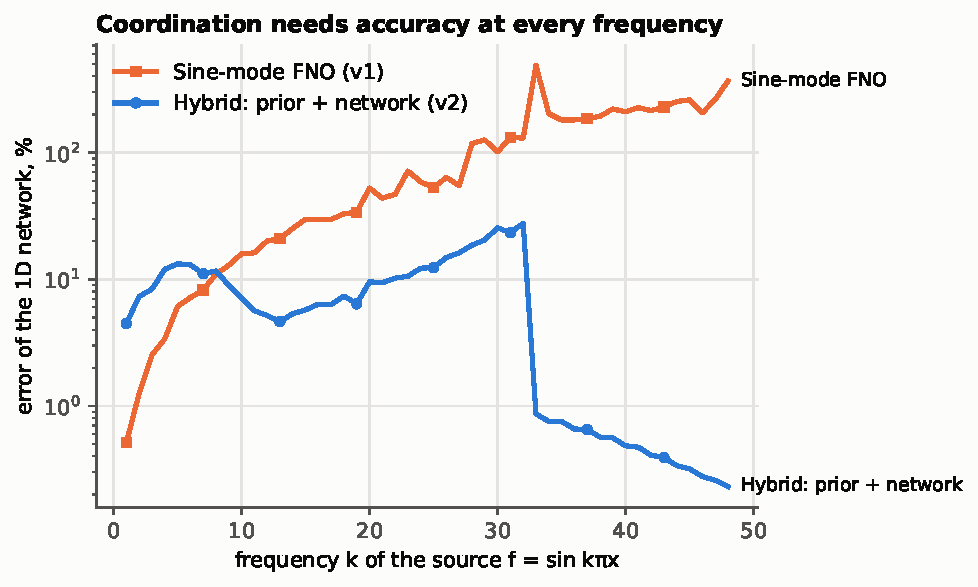
\includegraphics[width=0.62\linewidth]{fig3_frequency_lesson}
\caption{Error of the 1D surrogate for sources $\sin k\pi x$ ($n=48$). The sine-basis FNO is accurate
only for the lowest frequencies; the hybrid is accurate at high frequencies by construction, with
remaining error at intermediate ones.}
\label{fig:freq}
\end{figure}

\paragraph{Residual refinement.}
The 1D error grows with the contrast of $c$ along the line ($1.2\%$, $5.3\%$, $17\%$, $36\%$ for contrast
$<5$, $5$--$20$, $20$--$50$, $50$--$200$), because the prior $P_0$ only freezes the coefficient locally.
Since applying the tridiagonal operator $A(c)$ is cheap, we use the network $N$ with $R$ steps of defect
correction, $w_{j+1} = w_j + N(c)\,(f - A(c)w_j/h^2)$, which keeps the map linear in $f$ and uses no exact
solve. With the network above this diverges for contrast above $\approx 50$ ($I-NA$ is not a contraction).
We therefore fine-tune $N$ through the unrolled refinement ($R=2$; loss $\log(1+e)$ over the errors after
$0,1,2$ steps; coefficient fields with $20$--$30\%$ larger $\log c$; 30\,000 steps, 9\,min). The refined
network reaches $0.01\%$, $0.1\%$, $1.1$--$1.4\%$ and $15\%$ for the same contrast bands, at any line length
($48$--$198$); above contrast $200$ it still diverges. We call it v3 and the network without refinement v2.

\paragraph{Preconditioner.}
A ``coarse model'' preconditioner uses the exact inverse of the coordination Jacobian for the
constant coefficient $\bar k$: $P = \bar k h^{-2}\, T_y (T_x+T_y)^{-1} T_x$, with $(T_x+T_y)^{-1}$
approximated by ADI in 2D and applied exactly by a 3D sine transform in 3D. It does not look inside the
surrogate and does not change the answer; for the first (fixed-length) network it reduced GMRES
iterations from 545 to 60.

\section{Results}

\paragraph{2D, variable coefficient, several grids.}
For $-\nabla\cdot(k\nabla\varphi)=0$ with three unseen coefficient fields and three boundary-condition
types (constant and sinusoidal top boundary, constant right boundary plus a bump at the bottom), the
reference is the same coordination with exact Thomas solves, which reproduces the five-point scheme to
$3\cdot10^{-13}$. The mean (worst) error is $0.56\%$ ($1.20\%$), $0.55\%$ ($1.16\%$), $0.55\%$ ($1.14\%$) on
$50^2$, $100^2$, $200^2$, with 17--23 GMRES iterations independent of the grid. With the refined network
(v3) the same 27 problems give $0.002\%$ mean error (worst $0.006\%$) on every grid, with the same iteration counts; the network part
then costs about as much as exact Thomas solves (e.g.\ $0.6$\,s vs.\ $0.5$\,s on $100^2$).

\paragraph{3D.}
The same network, without retraining, solves the 3D problem along $x$, $y$ and $z$ lines. On $24^3$,
$48^3$, $96^3$ grids (six problems each) the mean error is $0.49\%$, $0.39\%$, $0.36\%$ (worst $0.89\%$)
with 16--22 iterations (Figure~\ref{fig:grids}). On a laptop CPU the $96^3$ problem
($8.8\cdot10^5$ unknowns) takes about 7\,s, versus 2.7\,s with exact Thomas solves: with an exact
1D solver available, the network is slower, as expected. With v3 the mean error is $0.0005\%$, $0.0003\%$, $0.0002\%$ (worst
$0.0006\%$), at a higher cost: $23$--$31$\,s on $96^3$ (three network applications per line solve)
versus $3$--$4$\,s with Thomas.

\begin{figure}[t]
\centering
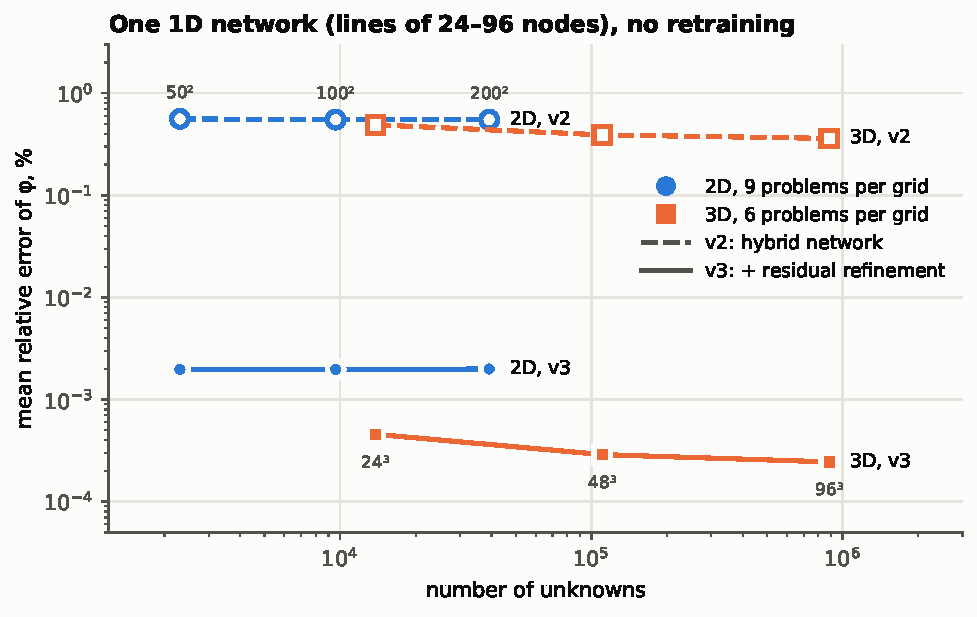
\includegraphics[width=0.62\linewidth]{fig2_grid_independence}
\caption{Mean error of coordination with one 1D network (trained on lines of 24--96 nodes) on 2D and
3D grids (logarithmic scale): hybrid network (v2, dashed) and the same network with two residual-refinement
steps (v3, solid). The error does not grow with the grid. No 2D or 3D data was used in training.}
\label{fig:grids}
\end{figure}

\paragraph{Out-of-distribution coefficients.}
With the first (fixed-length) network, 30 unseen problems with coefficient contrast $3$--$35$ gave
$0.3$--$1.4\%$ error; contrast $340$--$380$, outside the training range, gave up to $12\%$, again
matching the 1D error rather than amplifying it.

\section{A learned atmospheric column with chemistry}
\label{sec:chem}

We consider a vertical cross-section of the atmosphere,
\begin{equation}
  -(k\varphi_x)_x - (K\varphi_z)_z + \sigma\,\varphi|\varphi| = s,
\end{equation}
with a stack source near the ground and an area source, vertical eddy diffusivity $K(x,z)$ that is
small near the ground and peaks in the boundary layer, and a second-order reaction with rate $\sigma(x)$.
Horizontal lines are solved exactly (linear); vertical columns, which carry the nonlinear chemistry,
are solved by a network. Without the network each column requires Newton iterations.

\paragraph{Learned effective reaction rate.}
A network that outputs the column profile directly reached only $15$--$26\%$ column error. Instead,
the network predicts a smooth non-negative effective rate $\mu(z)\approx\sigma|v(z)|$ and the column is
obtained by one tridiagonal solve $(A + h^2\mu)v = h^2 g$; the exact $\mu$ reproduces the exact column
to $2\cdot10^{-14}$. Training data must match the regime met in the coupled problem: with chemistry
strength $\sigma|v|/(\pi^2K)$ mostly below $0.05$ in training, the coupled error was $21$--$24\%$ for strong
chemistry, and the error of the network on the \emph{true} columns of the section matched it
($3.8/12/22\%$ vs.\ $2.4/12/24\%$), confirming that coordination did not amplify it. Sampling the strength
log-uniformly (up to $\approx 50$) and including atmospheric $K$ profiles fixed this.

\begin{table}[t]
\centering
\caption{Atmospheric section: relative error of the coupled solution with a learned chemistry column.}
\label{tab:chem}
\begin{tabular}{lrrrr}
\toprule
chemistry ($\sigma_0$; share of balance) & $50^2$ & $100^2$ & $200^2$ & Newton steps\\
\midrule
none (0; 0\%) & 0.00\% & 0.00\% & 0.00\% & 2\\
weak (5; 8\%) & 0.22\% & 0.19\% & 0.13\% & 6\\
medium (50; 30\%) & 1.39\% & 1.16\% & 1.06\% & 5\\
strong (300; 54\%) & 3.82\% & 3.66\% & 3.93\% & 7--10\\
\bottomrule
\end{tabular}
\end{table}

\begin{figure}[t]
\centering
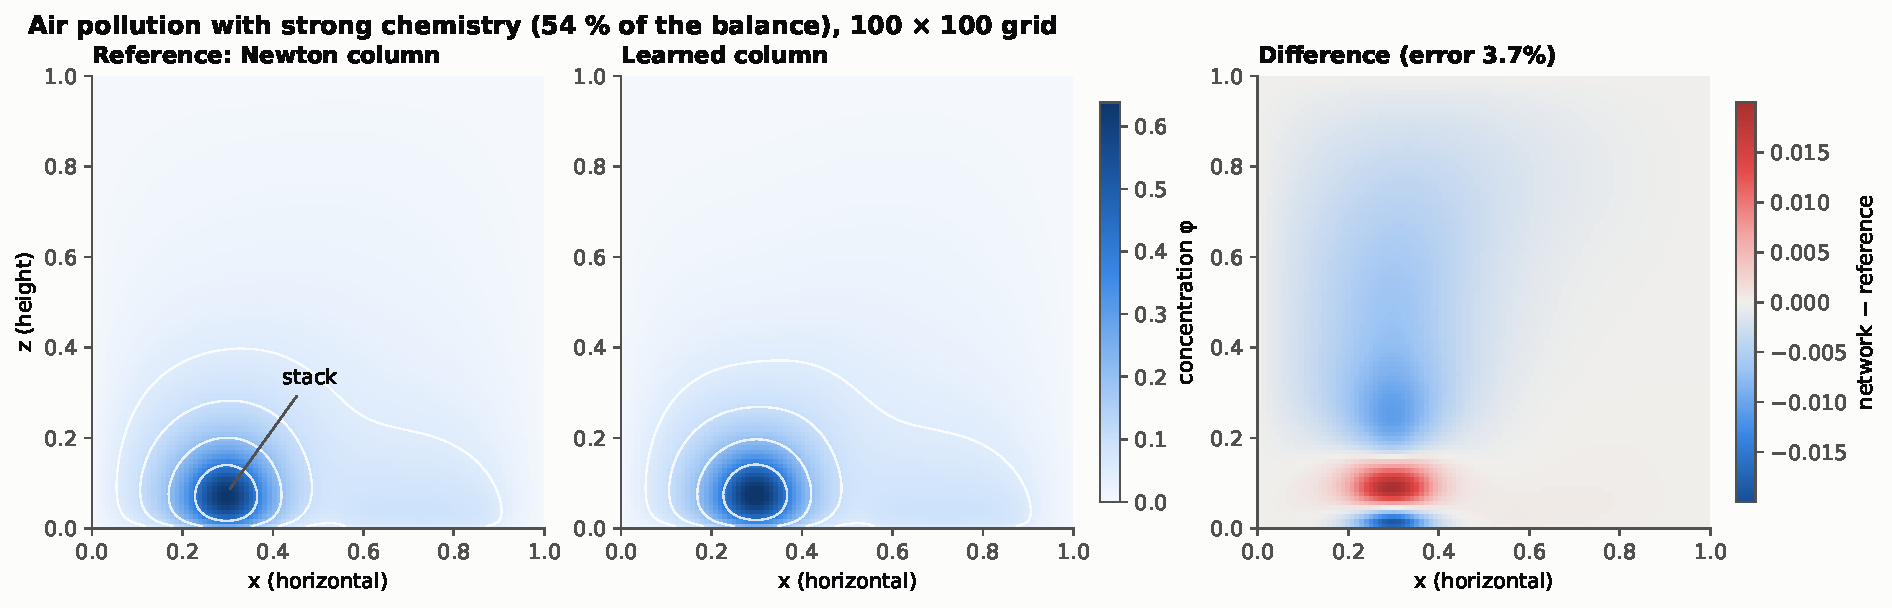
\includegraphics[width=\linewidth]{fig1_pollution_section}
\caption{Pollutant concentration with strong chemistry on a $100\times100$ grid: reference with Newton
columns, learned columns, and their difference.}
\label{fig:section}
\end{figure}

A single learned column is 2--6 times faster than a Newton column (1024 columns: 11--17\,ms vs.\
24--95\,ms), but the full coupled solve is currently slower than the exact one because of the
Newton--Krylov overhead in our Python implementation.

\section{Three reacting species: a learned warm start for Newton}
\label{sec:multi}

To move towards realistic atmospheric chemistry we replace the single reaction by the classical
NO--NO$_2$--O$_3$ cycle with removal terms. With $c=(a,b,o)$ the concentrations of NO, NO$_2$ and O$_3$,
\begin{align}
  -\nabla\cdot(K\nabla a) + k\,a\,o - J\,b &= s_a,\nonumber\\
  -\nabla\cdot(K\nabla b) - k\,a\,o + (J+\lambda)\,b &= s_b,\\
  -\nabla\cdot(K\nabla o) + k\,a\,o - J\,b + \delta\,o &= s_o,\nonumber
\end{align}
where $J$ is the photolysis rate of NO$_2$, $k$ the rate of the titration reaction NO + O$_3$ $\to$ NO$_2$,
$\lambda$ the removal of NO$_2$ and $\delta$ the loss of ozone. The loss terms break the two conservation laws
of the bare cycle (NO$_x$ and O$_x$), so the three species do not reduce to a single scalar equation. Rows
(horizontal, linear) are solved exactly for each species; each vertical column is a nonlinear system with
$3\times3$ blocks, solved exactly by Newton's method with block-tridiagonal factorisations.

\paragraph{Column network.}
The only nonlinear term is $k\,a\,o$. The network predicts a smooth ozone profile $\hat o(z)$ from cosine
features of $\log K$, non-dimensional rates and the low sine modes of the column solution without the
titration reaction (one block solve). With $k\,a\,o$ replaced by $k\,\hat o\,a$ the column is linear and is
solved by one block-tridiagonal solve; it is exact if $\hat o$ is. The network is trained for 6 minutes on
49\,000 exact columns of 24--64 nodes.

\paragraph{Refinement: Picard fails, Newton works.}
Refining by Picard iteration ($\hat o \leftarrow o$) diverges in NO-rich columns, where ozone is almost fully
titrated (near stacks and roads): the mean error after two steps was $1400\%$. Freezing the nonlinearity
differently in the ozone equation ($k\,\hat a\,o$, so that ozone keeps its own loss term) converges, but slowly
(mean $5$--$9\%$). Instead we take the network output as the starting point of Newton's method. Each Newton
step costs one block solve, like a Picard step, and from the learned start Newton converges quadratically
(Table~\ref{tab:multi}).

\begin{table}[t]
\centering
\caption{Single columns (1024 unseen random columns): relative error after the learned start plus $j$ Newton
steps (median / 99th percentile / worst) and time for all 1024 columns, compared with Newton's method from
zero with line search until convergence.}
\label{tab:multi}
\begin{tabular}{rlrr}
\toprule
nodes & method & error (median / 99\% / worst) & time\\
\midrule
48 & network only & $2.8\cdot10^{-3}$ / $4.9$ / $16$ & 33 ms\\
48 & network + 2 Newton & $1.8\cdot10^{-14}$ / $3.7\cdot10^{-4}$ / $2.4\cdot10^{-2}$ & 61 ms\\
48 & network + 3 Newton & $6.1\cdot10^{-15}$ / $1.1\cdot10^{-7}$ / $1.1\cdot10^{-4}$ & 80 ms\\
48 & Newton from zero, 3 steps & $1.0\cdot10^{-5}$ / $0.66$ / $3.3$ & --\\
48 & Newton from zero, converged & exact & 154 ms\\
\midrule
98 & network + 3 Newton & $1.8\cdot10^{-14}$ / $9.7\cdot10^{-7}$ / $4.7\cdot10^{-4}$ & 151 ms\\
98 & Newton from zero, 3 steps & $1.6\cdot10^{-5}$ / $0.74$ / $2.5$ & --\\
98 & Newton from zero, converged & exact & 490 ms\\
\bottomrule
\end{tabular}
\end{table}

The learned start saves two to three Newton steps and makes the column solve 1.9 (48 nodes) to 3.2 (98 nodes)
times faster at the same accuracy. Note that the network output alone has a heavy tail of errors (worst
columns $>100\%$); its value lies in being a good starting point, not in being a final answer.

\paragraph{Coupled section.}
In the cross-section of Section~\ref{sec:chem} with an NO stack, NO traffic emissions near the ground,
a background ozone source and photolysis varying along $x$, coordination with the learned start plus three
Newton steps per column reproduces the exact coupled solution to $10^{-14}$ (titration rate $k\le20$) and
$10^{-10}$ ($k=50$, titration $27\%$ of the balance) on $50^2$ and $100^2$ grids, with the same numbers of outer
Newton steps (2--5) and GMRES iterations (62--369). The column Jacobian used by GMRES is the exact one,
evaluated at the column state. The wall time, however, is unchanged ($20.3$\,s vs.\ $21.2$\,s on $100^2$,
$k=50$): column solves take less than $3\%$ of the run time, which is dominated by the GMRES coupling
iterations. For $k=300$ even the exact coordination does not converge with our preconditioner, which ignores
the chemistry.

This is a property of the steady-state setting, in which the coupling between columns and rows is solved
iteratively. In time-dependent chemical transport models with operator splitting, column chemistry is solved
independently at every time step and typically dominates the run time, with tens to hundreds of species; this
is where a learned warm start for the column Newton solve is expected to pay off.

\section{Comparison with a 2D neural operator}
\label{sec:baseline}
We compare against a standard 2D Fourier neural operator~\cite{li2021fno} (4 spectral layers, width 32,
12 modes, $1.2\cdot10^6$ parameters) that maps $(\log k$, boundary frame, frame mask$)$ on a $50\times50$ grid
to $\varphi$. It is trained on 1000 reference 2D solutions (358\,s to generate) for 900\,s, four times the
training budget of the 1D network. The problem family is the same for both methods: random smooth
coefficient fields with contrast $\max k/\min k$ between about 2 and 80 (median 9), and random smooth
boundary data. Applied directly on other grids, the FNO fails ($86$--$98\%$ error) because the one-cell
boundary frame changes meaning with resolution; we therefore report the stronger variant that resamples the
input to $50^2$ and interpolates the output back.

\begin{table}[t]
\centering
\caption{Mean (worst) relative error over 20 unseen problems per row, and wall time per problem.
FNO 2D is trained on $50^2$ 2D solutions; coordination uses the 1D network of Section~\ref{sec:hybrid},
trained on 1D lines only.}
\label{tab:baseline}
\begin{tabular}{llrrrr}
\toprule
test & grid & FNO 2D & coordination & FNO time & coord.\ time\\
\midrule
in distribution & $50^2$ & 3.65\% (7.1) & 0.13\% (2.3) & 11 ms & 0.54 s\\
other grid & $100^2$ & 4.08\% (10.2) & 0.05\% (0.3) & 13 ms & 0.92 s\\
other grid & $200^2$ & 3.50\% (7.1) & 0.06\% (0.4) & 47 ms & 2.11 s\\
step boundary data & $50^2$ & 9.91\% (14.8) & 0.13\% (1.4) & 8 ms & 0.54 s\\
step boundary data & $100^2$ & 9.47\% (17.1) & 0.71\% (13.1) & 14 ms & 1.22 s\\
\midrule
\multicolumn{6}{l}{without refinement (v2): $2.27/2.15/2.05/2.29/2.31\%$ mean, worst $15.0\%$}\\
\bottomrule
\end{tabular}
\end{table}

Table~\ref{tab:baseline} uses the refined 1D network (v3). Coordination is 30--180 times more accurate on
average than the FNO in every setting, including other grids and boundary data of a kind not seen in
training: the boundary values enter the 1D subproblems exactly, whereas the 2D network must learn their
effect. Without refinement (v2) the advantage was smaller ($2.1$--$2.3\%$) and the worst case ($15\%$) was
worse than the FNO's. The one remaining outlier ($13.1\%$, step data on $100^2$) contains a grid line with
coefficient contrast $52$, where the refined 1D network has $\approx15\%$ error; GMRES needed 180 iterations
instead of the usual 20--30. The FNO is 40--60 times faster at inference. The coordination approach needs no
2D data at all.

\section{Limitations and outlook}

\begin{itemize}
  \item With exact 1D solvers the method is not faster than ADI-preconditioned GMRES or a direct
        solver; benefits appear only when the 1D model is expensive or unavailable in closed form.
  \item The hybrid 1D network still has $5$--$27\%$ error at intermediate frequencies; better
        architectures or training in the residual norm should reduce the assembled error.
  \item The chemistry demonstrations use one and three species and a steady state. In the steady coupled
        problem column solves are a small part of the run time, so the faster columns of
        Section~\ref{sec:multi} do not shorten the whole computation. A time-dependent model with
        operator splitting and a larger mechanism, where column chemistry dominates, is the natural next
        test, as is a GPU implementation in which all lines of a direction are solved as one batch.
  \item Our coarse preconditioner ignores the chemistry; for fast titration ($k=300$) the coordination does
        not converge even with exact columns.
  \item Novelty of the dimension-splitting coordination itself should be assessed against the
        virtual-control literature of Lions and Pironneau, which explicitly proposes the decomposition of operators~\cite{lions1998,lions2000}, and optimization-based domain decomposition~\cite{gunzburger2000}.
\end{itemize}

\paragraph{Acknowledgements.}
The author thanks the originator of the coordination method for the idea and for discussions.
An AI assistant was used for writing code and drafting the text; all results were checked by the authors.

\paragraph{Reproducibility.}
All experiments run on a laptop CPU in PyTorch; scripts \texttt{surrogate\_error\_robustness.py},
\texttt{nn\_coordination.py}, \texttt{nn\_generalize.py}, \texttt{nn\_coordination\_grids.py}, \texttt{nn\_line\_refined.py},
\texttt{nn\_coordination\_3d.py}, \texttt{nn\_column\_chemistry.py}, \texttt{nn\_column\_multispecies.py}, \texttt{baseline\_fno2d.py} and
\texttt{make\_figures.py} reproduce every number and figure; logs are in \texttt{results/}.

\bibliographystyle{unsrtnat}
\bibliography{refs}
\end{document}
